\chapter{HASIL \textit{CONFERENCE POPULARITY ANALYSIS}}
\label{chap:popularitas}\label{sec:hasil-t2}

\section{Sepuluh Konferensi Teratas}
\label{sec:hasil-top}
Popularitas diukur dengan dua ukuran. Jumlah publikasi menghitung makalah yang diterbitkan konferensi, sedangkan jumlah penulis unik menghitung orang berbeda yang pernah menerbitkan di sana, dengan satu orang dihitung sekali berapa pun jumlah makalahnya. Kedua ukuran dihitung dari seluruh periode 2015--2025.

Gambar~\ref{fig:top-pub} dan Gambar~\ref{fig:top-author} menunjukkan sepuluh konferensi dengan publikasi terbanyak dan penulis unik terbanyak.
\begin{enumerate}
\item NeurIPS berada di peringkat pertama pada kedua ukuran (25.455 makalah atau 1,27\% \textit{dataset}, dan 57.800 penulis unik), disusul CVPR (22.751; 47.664) dan ICASSP (21.606; 42.057).
\item Delapan dari sepuluh konferensi sama pada kedua daftar. CHI dan ICC hanya masuk pada daftar publikasi, sedangkan ICML (31.896 penulis) dan IROS (31.249) hanya masuk pada daftar penulis unik.
\item Sepuluh konferensi teratas menghasilkan 9,4\% seluruh publikasi dan berasal dari bidang yang beragam, yaitu kecerdasan buatan dan pemrosesan bahasa alami, sinyal dan penginderaan jauh, interaksi manusia-komputer, serta biomedis dan komunikasi.
\end{enumerate}

\begin{figure}[!htb]
\centering
\figtikz[9.2cm]{fig-top10-publikasi}
\caption{Sepuluh konferensi dengan publikasi terbanyak}
\label{fig:top-pub}
\end{figure}

\begin{figure}[!htb]
\centering
\figtikz[9.2cm]{fig-top10-author}
\caption{Sepuluh konferensi dengan penulis unik terbanyak}
\label{fig:top-author}
\end{figure}

\section{Tren Publikasi}
\label{sec:hasil-tren}
Tren dihitung untuk 2015--2024 karena 2025 belum lengkap. Pertumbuhan diringkas dengan \textit{compound annual growth rate} (CAGR), yaitu laju pertumbuhan tahunan rata-rata dari 2015 ke 2024, dan diperlihatkan sebagai kelipatan jumlah makalah.

Gambar~\ref{fig:tren-top10} menunjukkan tren sepuluh konferensi teratas dan Gambar~\ref{fig:cagr} laju pertumbuhannya.
\begin{enumerate}
\item NeurIPS, EMNLP, CVPR, dan AAAI tumbuh 10,2, 7,6, 4,8, dan 3,6 kali dari 2015 ke 2024, jauh di atas CAGR seluruh \textit{dataset} (3,2\%).
\item HCI hampir datar, sedangkan ICC dan EMBC menurun.
\item Porsi sepuluh konferensi teratas terhadap seluruh publikasi naik dari 7,0\% (2015) menjadi 11,7\% (2024), sehingga aktivitas makin terkonsentrasi.
\end{enumerate}

\begin{figure}[!htb]
\centering
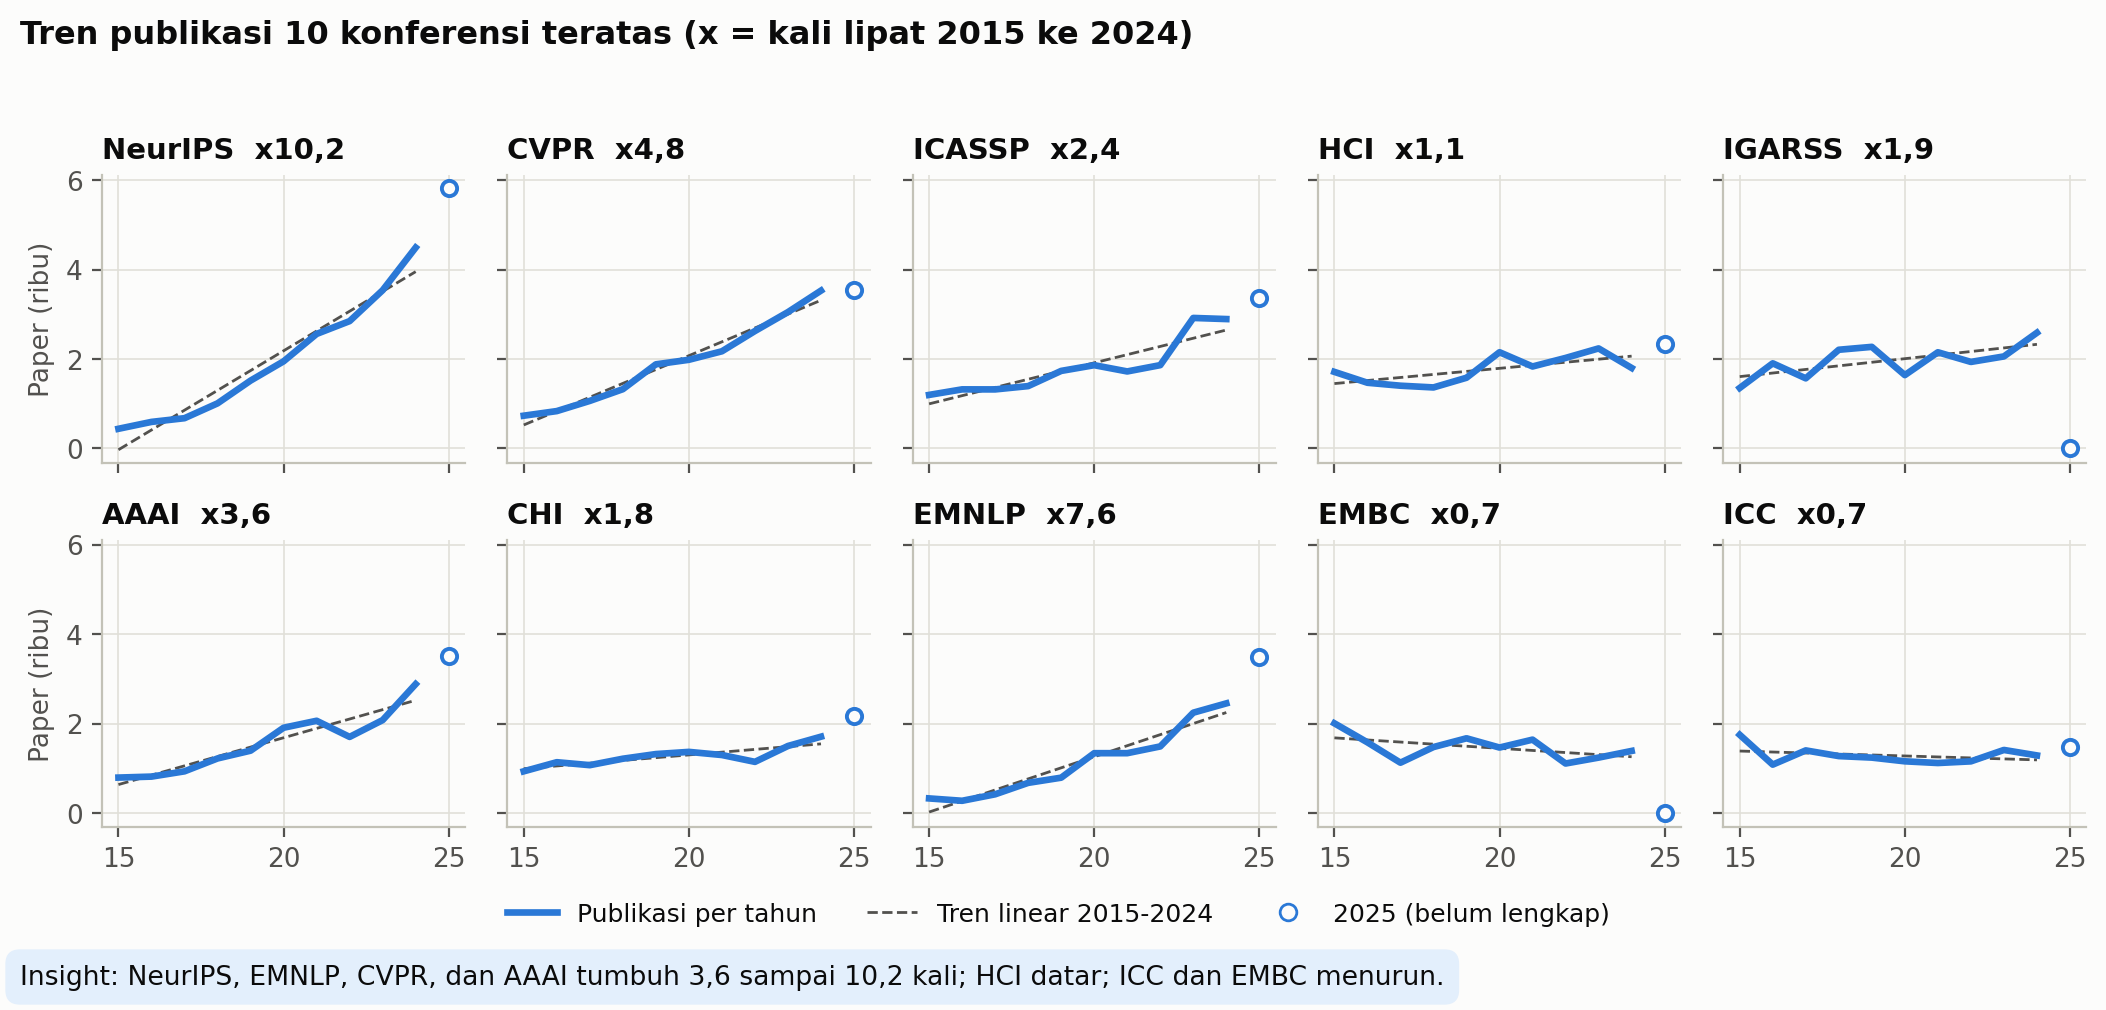
\includegraphics[width=\textwidth]{images/hasil/t2_tren_top10.png}
\caption{Tren publikasi per tahun pada sepuluh konferensi teratas}
\label{fig:tren-top10}
\end{figure}

\begin{figure}[!htb]
\centering
\figtikz[9cm]{fig-cagr-top10}
\caption{Laju pertumbuhan tahunan (CAGR) sepuluh konferensi teratas, 2015--2024}
\label{fig:cagr}
\end{figure}

\section{Perbandingan Peringkat}
\label{sec:hasil-banding}
Tabel~\ref{tab:banding} membandingkan peringkat kedua ukuran, dengan selisih positif berarti naik pada peringkat penulis unik. Kedua peringkat sangat selaras: korelasi Spearman pada 4.373 \textit{venue} mencapai 0,987, dan hampir semua konferensi berada pada sekitar dua penulis unik per makalah (Gambar~\ref{fig:scatter}). Perbedaan terjadi pada peringkat tengah. AAAI dan EMBC naik karena menarik lebih banyak penulis berbeda per makalah, sedangkan CHI dan ICC turun, dengan ICC turun paling jauh (sepuluh ke sembilan belas).

\begin{table}[!htb]
\caption{Perbandingan peringkat publikasi dan penulis unik}
\label{tab:banding}
\small
\begin{tabular*}{\textwidth}{@{\extracolsep{\fill}}@{}lrrr@{}}
\toprule
\textbf{Konferensi} & \textbf{Peringkat publikasi} & \textbf{Peringkat penulis unik} & \textbf{Selisih} \\
\midrule
NeurIPS & 1 & 1 & 0 \\
CVPR & 2 & 2 & 0 \\
ICASSP & 3 & 4 & $-$1 \\
HCI & 4 & 6 & $-$2 \\
IGARSS & 5 & 7 & $-$2 \\
AAAI & 6 & 3 & $+$3 \\
CHI & 7 & 12 & $-$5 \\
EMNLP & 8 & 8 & 0 \\
EMBC & 9 & 5 & $+$4 \\
ICC & 10 & 19 & $-$9 \\
ICML & 12 & 9 & $+$3 \\
IROS & 14 & 10 & $+$4 \\
\bottomrule
\end{tabular*}
\end{table}

\begin{figure}[!htb]
\centering
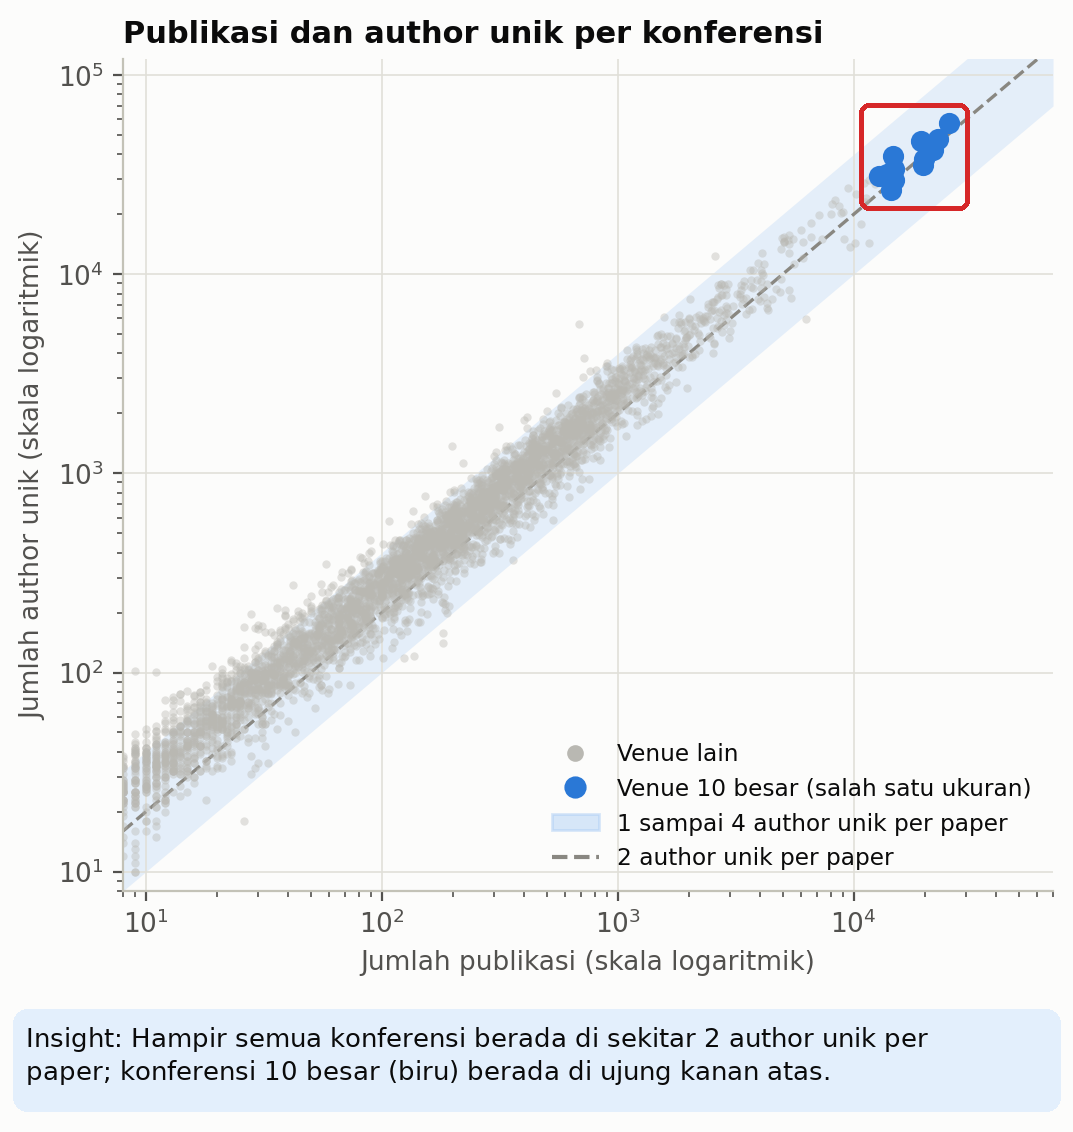
\includegraphics[width=0.62\textwidth]{images/hasil/t2_scatter_publikasi_author.png}
\caption{Publikasi dan penulis unik per konferensi}
\label{fig:scatter}
\end{figure}

\section{Uji Sensitivitas terhadap \textit{Workshop}}
\label{sec:hasil-sensitivitas}
\textit{Workshop} yang memakai \textit{key} konferensi induk ikut terhitung sebagai konferensi induknya (Subbab~\ref{sec:key}). Untuk menguji dampaknya, peringkat dihitung ulang tanpa \textit{workshop} dan acara pendamping, yang dikenali dari kata kunci pada \textit{booktitle} (misalnya \textit{Workshop}, \textit{Extended Abstracts}, \textit{Companion}) dan mencakup 7,2\% makalah. Tabel~\ref{tab:sensitivitas} menunjukkan bahwa peringkat teratas relatif kuat: NeurIPS tetap nomor satu dan delapan dari sepuluh konferensi teratas tetap sama. Konferensi dengan banyak \textit{workshop} paling terpengaruh, yaitu CVPR (\textit{CVPR Workshops}), ICC, dan CHI (\textit{CHI Extended Abstracts}). Karena itu pernyataan bahwa CVPR adalah konferensi terpopuler kedua bergantung pada definisi, dan laporan ini memakai definisi berbasis \textit{key}.

\begin{table}[!htb]
\caption{Peringkat publikasi dengan dan tanpa \textit{workshop}}
\label{tab:sensitivitas}
\small
\begin{tabular*}{\textwidth}{@{\extracolsep{\fill}}@{}lrrr@{}}
\toprule
\textbf{Konferensi} & \textbf{Peringkat awal} & \textbf{Peringkat tanpa \textit{workshop}} & \textbf{Porsi \textit{workshop}} \\
\midrule
NeurIPS & 1 & 1 & 1,1\% \\
CVPR & 2 & 6 & 23,4\% \\
ICASSP & 3 & 2 & 2,2\% \\
CHI & 7 & 29 & 44,0\% \\
ICC & 10 & 18 & 22,8\% \\
ICML & 12 & 9 & 0,6\% \\
\bottomrule
\end{tabular*}
\end{table}
